% =============================================================================
%  COMPUTATIONAL RESULTS — revised draft (rewrite of 2026-08-03)
%
%  Regenerated against the runs of 2026-08-03:
%     tables/gap.tex, gap_nopen.tex, feasibility.tex, runtime.tex
%     tables/additional_diesel.tex, additional_sensitivity.tex
%     figures/paper_gap_stats.csv, additional_sens_stats.csv,
%     figures/additional_diesel_stats.csv
%
%  Scope per instruction: NO sensitivity on travel-time CV, on the window
%  penalty beta, on battery capacity, and NO Gamma (price-of-robustness)
%  frontier.  Those rows/figures are removed, not merely marked pending.
%
%  Conventions:  plain text = number verified against a stored result file
%                \red{...}  = still pending a run, or a decision for you
% =============================================================================

\subsection{Base-case comparison}
\label{sec:basecase}

Each instance class is instantiated with 50 independent random realizations,
and every realization is solved by all five methods (Greedy, RO, ROBU, LA, SP)
and evaluated in the common discrete-event simulator of
Section~\ref{sec:simulation} against the perfect-hindsight oracle.  Coverage is
now complete on the short and medium route classes for Greedy, RO, LA and SP;
on the long routes RO and LA are also complete or nearly so, whereas SP does
not terminate within its budget and ROBU terminates only on the short routes.
The tables and figures draw the full canonical grid with the missing slots left
empty rather than silently dropping them.

We compare the methods along three metrics.  First, efficiency, shown through
the gap to oracle in realized route duration in Table~\ref{tab:gap} and
Figure~\ref{fig:resultsgap}.  Then, reliability, via the rate at which the
executed schedule becomes infeasible (the infeasibility strip of
Figure~\ref{fig:resultsgap} and Table~\ref{tab:feasibility}).  Finally,
computational effort in Table~\ref{tab:runtime}.

Because the oracle is itself a mixed-integer program, the reference against
which every gap is measured is only as tight as its own certificate.
Figure~\ref{fig:boundsoracle} reports, per route class, the incumbent and the
best dual bound of the oracle solves.  On short and medium routes the oracle
closes to within \red{XX\%}.  On the long routes the incumbent stabilizes early
while the dual bound sometimes stalls at roughly 9\%.  Long-route gaps in
Table~\ref{tab:gap} are therefore not exact distances to the proved optimum,
but distances to the best incumbent, which we believe to be close to it.

\begin{table}[htbp]
\centering
\caption{Gap to oracle (\%) in route duration (window penalties included) by instance class and method, averaged over 50 realizations per instance class.  Parentheses give the same gap over the same runs with window penalties excluded (route duration only).  ROBU is solved on the short-route instances only.  LA uses 25 scenarios over a 24\,h horizon; SP uses 25 scenarios.}
\label{tab:gap}
\resizebox{\textwidth}{!}{%
\begin{tabular}{lll c ccccc}
\toprule
\multirow{2}{*}{\textbf{\small Route}} & \multirow{2}{*}{\textbf{\small Cust.}} & \multirow{2}{*}{\textbf{\small TW}} & \multirow{2}{*}{\textbf{Oracle (h)}} &
\multicolumn{5}{c}{\textbf{Gap to Oracle \%}} \\
\cmidrule(lr){5-9}
 & & & & Greedy & RO & ROBU & LA & SP \\
\midrule
\multirow{12}{*}{\small Short} & \multirow{4}{*}{\small Few} & {\small None} & 26.5 & 12.4~{\scriptsize(12.4)} & 21.4~{\scriptsize(21.4)} & 14.1~{\scriptsize(14.1)} & 6.8~{\scriptsize(6.8)} & 3.7~{\scriptsize(3.7)} \\
 &  & {\small Tight} & 26.1 & 19.0~{\scriptsize(13.2)} & 27.2~{\scriptsize(21.6)} & 15.8~{\scriptsize(10.6)} & 10.3~{\scriptsize(7.2)} & 4.3~{\scriptsize(3.3)} \\
 &  & {\small Medium} & 26.3 & 16.9~{\scriptsize(12.7)} & 23.7~{\scriptsize(19.7)} & 16.1~{\scriptsize(13.4)} & 10.2~{\scriptsize(7.3)} & 4.0~{\scriptsize(3.9)} \\
 &  & {\small Large} & 26.2 & 15.7~{\scriptsize(13.3)} & 22.2~{\scriptsize(19.2)} & 14.3~{\scriptsize(12.7)} & 8.9~{\scriptsize(6.6)} & 4.0~{\scriptsize(3.9)} \\
 & \multirow{4}{*}{\small Medium} & {\small None} & 28.0 & 11.9~{\scriptsize(11.9)} & 20.9~{\scriptsize(20.9)} & 16.1~{\scriptsize(16.1)} & 8.8~{\scriptsize(8.8)} & 4.3~{\scriptsize(4.3)} \\
 &  & {\small Tight} & 28.0 & 28.2~{\scriptsize(12.8)} & 36.9~{\scriptsize(23.9)} & 27.7~{\scriptsize(15.0)} & 15.2~{\scriptsize(6.9)} & 5.7~{\scriptsize(3.2)} \\
 &  & {\small Medium} & 27.6 & 21.2~{\scriptsize(13.0)} & 30.6~{\scriptsize(20.6)} & 19.0~{\scriptsize(12.0)} & 11.6~{\scriptsize(7.1)} & 4.6~{\scriptsize(4.1)} \\
 &  & {\small Large} & 28.2 & 16.6~{\scriptsize(12.1)} & 34.0~{\scriptsize(26.8)} & 24.2~{\scriptsize(20.3)} & 11.5~{\scriptsize(7.2)} & 3.6~{\scriptsize(3.5)} \\
 & \multirow{4}{*}{\small Many} & {\small None} & 31.3 & 13.9~{\scriptsize(13.9)} & 26.8~{\scriptsize(26.8)} & 22.0~{\scriptsize(22.0)} & 5.8~{\scriptsize(5.8)} & 4.7~{\scriptsize(4.7)} \\
 &  & {\small Tight} & 31.4 & 41.9~{\scriptsize(14.0)} & 52.0~{\scriptsize(26.6)} & 45.8~{\scriptsize(22.7)} & 17.0~{\scriptsize(8.1)} & 10.4~{\scriptsize(4.2)} \\
 &  & {\small Medium} & 31.7 & 33.4~{\scriptsize(15.4)} & 48.0~{\scriptsize(27.2)} & 36.4~{\scriptsize(21.9)} & 21.9~{\scriptsize(12.6)} & 5.2~{\scriptsize(4.0)} \\
 &  & {\small Large} & 30.5 & 16.5~{\scriptsize(11.0)} & 39.0~{\scriptsize(26.8)} & 24.2~{\scriptsize(19.4)} & 11.8~{\scriptsize(7.9)} & 3.9~{\scriptsize(3.4)} \\
\midrule
\multirow{12}{*}{\small Medium} & \multirow{4}{*}{\small Few} & {\small None} & 54.5 & 16.3~{\scriptsize(16.3)} & 37.0~{\scriptsize(37.0)} & -- & 10.6~{\scriptsize(10.6)} & 12.5~{\scriptsize(12.5)} \\
 &  & {\small Tight} & 56.0 & 17.1~{\scriptsize(13.4)} & 33.7~{\scriptsize(30.8)} & -- & 10.0~{\scriptsize(7.6)} & 10.9~{\scriptsize(9.1)} \\
 &  & {\small Medium} & 54.1 & 16.7~{\scriptsize(14.1)} & 36.1~{\scriptsize(32.9)} & -- & 10.6~{\scriptsize(9.1)} & 8.5~{\scriptsize(7.9)} \\
 &  & {\small Large} & 54.5 & 14.0~{\scriptsize(13.1)} & 34.1~{\scriptsize(31.0)} & 53.7~{\scriptsize(50.9)} & 9.4~{\scriptsize(8.7)} & 8.0~{\scriptsize(7.6)} \\
 & \multirow{4}{*}{\small Medium} & {\small None} & 57.3 & 12.6~{\scriptsize(12.6)} & 30.1~{\scriptsize(30.1)} & -- & 8.1~{\scriptsize(8.1)} & 10.2~{\scriptsize(10.2)} \\
 &  & {\small Tight} & 56.2 & 21.6~{\scriptsize(13.2)} & 36.4~{\scriptsize(28.3)} & -- & 14.9~{\scriptsize(8.4)} & 13.9~{\scriptsize(9.1)} \\
 &  & {\small Medium} & 55.8 & 19.7~{\scriptsize(13.1)} & 38.8~{\scriptsize(30.8)} & -- & 13.6~{\scriptsize(8.9)} & 11.9~{\scriptsize(9.0)} \\
 &  & {\small Large} & 55.0 & 15.5~{\scriptsize(13.0)} & 36.8~{\scriptsize(30.0)} & -- & 9.9~{\scriptsize(8.3)} & 10.8~{\scriptsize(10.2)} \\
 & \multirow{4}{*}{\small Many} & {\small None} & 60.2 & 13.1~{\scriptsize(13.1)} & 27.1~{\scriptsize(27.1)} & -- & 9.0~{\scriptsize(9.0)} & 10.2~{\scriptsize(10.2)} \\
 &  & {\small Tight} & 60.2 & 32.5~{\scriptsize(14.6)} & 43.9~{\scriptsize(26.9)} & -- & 25.2~{\scriptsize(10.9)} & 26.2~{\scriptsize(13.9)} \\
 &  & {\small Medium} & 60.3 & 27.6~{\scriptsize(14.6)} & 40.3~{\scriptsize(26.6)} & -- & 20.3~{\scriptsize(11.9)} & 17.4~{\scriptsize(12.8)} \\
 &  & {\small Large} & 58.9 & 18.9~{\scriptsize(13.1)} & 39.7~{\scriptsize(26.2)} & -- & 13.9~{\scriptsize(9.4)} & 14.9~{\scriptsize(12.1)} \\
\midrule
\multirow{12}{*}{\small Long} & \multirow{4}{*}{\small Few} & {\small None} & 102.8 & 11.3~{\scriptsize(11.3)} & 33.4~{\scriptsize(33.4)} & -- & 8.0~{\scriptsize(8.0)} & -- \\
 &  & {\small Tight} & 107.5 & 13.3~{\scriptsize(11.9)} & 35.7~{\scriptsize(34.3)} & -- & 10.1~{\scriptsize(8.9)} & -- \\
 &  & {\small Medium} & 105.5 & 13.6~{\scriptsize(12.0)} & 36.3~{\scriptsize(34.6)} & -- & 11.0~{\scriptsize(9.8)} & 28.3~{\scriptsize(26.6)} \\
 &  & {\small Large} & 104.8 & 11.9~{\scriptsize(11.3)} & 35.7~{\scriptsize(34.1)} & -- & 8.4~{\scriptsize(8.0)} & 18.9~{\scriptsize(17.9)} \\
 & \multirow{4}{*}{\small Medium} & {\small None} & 104.8 & 11.6~{\scriptsize(11.6)} & 32.1~{\scriptsize(32.1)} & -- & 8.6~{\scriptsize(8.6)} & -- \\
 &  & {\small Tight} & 105.9 & 15.8~{\scriptsize(11.6)} & -- & -- & 12.1~{\scriptsize(8.7)} & -- \\
 &  & {\small Medium} & 105.6 & 15.0~{\scriptsize(11.2)} & 36.3~{\scriptsize(31.9)} & -- & 11.0~{\scriptsize(8.8)} & -- \\
 &  & {\small Large} & 104.3 & 13.3~{\scriptsize(11.9)} & 37.1~{\scriptsize(33.6)} & -- & 9.9~{\scriptsize(9.5)} & -- \\
 & \multirow{4}{*}{\small Many} & {\small None} & 108.2 & 11.9~{\scriptsize(11.9)} & 31.3~{\scriptsize(31.3)} & -- & 10.2~{\scriptsize(10.2)} & -- \\
 &  & {\small Tight} & 109.0 & 18.1~{\scriptsize(10.2)} & 38.1~{\scriptsize(29.7)} & -- & 17.0~{\scriptsize(10.5)} & -- \\
 &  & {\small Medium} & 113.3 & 14.1~{\scriptsize(10.1)} & 36.2~{\scriptsize(29.5)} & -- & 12.6~{\scriptsize(9.6)} & -- \\
 &  & {\small Large} & 110.7 & 13.0~{\scriptsize(10.9)} & 37.1~{\scriptsize(30.4)} & -- & 12.6~{\scriptsize(11.2)} & -- \\
\bottomrule
\end{tabular}%
}
\end{table}

\begin{figure}[htbp]
    \centering
    \includegraphics[width=\linewidth]{figures/boundsoracle.png}
    \caption{Convergence of the perfect-hindsight oracle for the medium route
    class: incumbent objective against the best dual bound over wall-clock
    time, one trace per instance.}
    \label{fig:boundsoracle}
\end{figure}

\begin{figure}[htbp]
    \centering
    \includegraphics[width=\linewidth]{figures/resultsgap.png}
    \caption{Distribution of the realized gap to the oracle across seeds, by
    route class, customer count, method (colour) and time-window class (shade,
    Tight--Medium--Large--None).  Boxes span the interquartile range, whiskers
    1.5\,IQR.  The heat strip below each panel shades the infeasibility rate.
    Empty slots are instance/method combinations without completed runs.}
    \label{fig:resultsgap}
\end{figure}

Across instance classes the two-stage stochastic plan (SP) and the look-ahead
policy (LA) attain the smallest gaps to the oracle (SP 3.6--26.2\%, mean 8.9\%;
LA 5.8--25.2\%, mean 11.8\%), the myopic greedy heuristic is intermediate
(11.7--42.8\%, mean 18.2\%), and the static robust plans are the most
conservative (ROBU 14.1--53.7\%, mean 25.3\%; RO 20.9--52.0\%, mean 34.5\%).
This ordering follows the amount of information each method uses and the point
at which it commits: the two policies that adapt to realized travel times (SP
through online duration recourse and LA through full re-optimisation at every
stop) recover most of the hindsight optimum, whereas the offline robust plans
pay for committing every duration in advance against a possible worst case.

The ordering between SP and LA reverses with route length.  On the short routes
SP is clearly ahead (4.9\% vs.\ 11.7\% on average), because 25 scenarios drawn
over the whole horizon still describe the realization well.  On the medium
routes the two are indistinguishable (12.9\% each), and on the long routes SP
no longer terminates at all, so LA (10.9\% on average) is the only adaptive
method that scales.  Greedy, conversely, improves in relative terms as routes
lengthen (21.3\%, 19.2\%, 13.7\% mean gap on short, medium and long routes): on
a 100\,h route the mandatory rest structure dominates the schedule and leaves
comparatively little for a planner to exploit.  RO shows no such trend
(31.9\%, 36.2\%, 35.7\%), which is expected of a plan priced at the worst-case
corner on every leg regardless of horizon.

The gap widens sharply with the number of customers and the tightness of the
windows.  On the short routes the \emph{Few}/\emph{Large} cell gives
16.3/22.2/14.3/8.9/4.0\% for Greedy/RO/ROBU/LA/SP against
42.8/52.0/45.8/17.0/10.4\% on \emph{Many}/\emph{Tight}: a two- to three-fold
deterioration for the three committing methods and roughly a doubling for the
two adaptive ones.  A static schedule that must satisfy more, and narrower,
service windows simultaneously is exactly the situation in which committing
early is most expensive.

A substantial part of the gap on the window-constrained classes is window
penalty rather than slower routing.  Comparing the penalized gap of
Table~\ref{tab:gap} with the duration-only gap in parentheses,
the $\beta\sum_i\delta_i$ term accounts on average for 16\% of RO's gap and
21\% of Greedy's, and on the tight-window classes for 25\% of RO's (range
4--49\%) against 38\% of Greedy's (9--66\%).  The penalty share is thus
\emph{smallest} for the box robust plan: RO is genuinely slower, spending its
gap on conservative durations, whereas Greedy's tight-window gap is mostly the
cost of arriving off the windows, up to two-thirds of it on
\emph{Short}/\emph{Many}/\emph{Tight} (42.8\% penalized against 14.5\%
duration-only).  The adaptive policies sit in between (LA 38\%, SP 38\% on
tight windows), consistent with policies that buy window compliance with a
little extra time.  On the window-free classes the two gap definitions coincide
exactly.

Where both static robust variants terminate, that is on the twelve short-route
classes, the budgeted plan (ROBU) improves on the box plan (RO) in every single
cell, by 4.8 to 14.8 percentage points (23.0\% vs.\ 31.9\% on average; e.g.\
19.0\% vs.\ 30.6\% on \emph{Short}/\emph{Medium}/\emph{Medium}).  This confirms
that pricing only a bounded number of legs at their worst case removes a large
part of the box's conservatism while retaining a guarantee
(Section~\ref{sec:robu}).

\begin{table}[htbp]
\centering
\caption{Feasibility and robustness statistics by method: HoS-violation rate, SOC-violation (stranding) rate, repair frequency (offline plans), and window hit rate, computed over runs whose plan the solver certified.  ``Not opt.'' is the share of runs returned at the time limit without a proven optimum and ``Opt.\ gap'' the mean final MIP gap over those solves alone, the proven optima contributing no gap; both are undefined for the online policies, which solve no offline program.  It averages the solver logs retained for RO 527 of 629, ROBU 0 of 55, SP 104 of 489 such solves.}
\label{tab:feasibility}
\resizebox{\textwidth}{!}{%
\begin{tabular}{lcccccc}
\toprule
\textbf{Method} & \textbf{HoS viol. (\%)} & \textbf{SOC viol. (\%)} & \textbf{Repairs (\%)} & \textbf{TW hit (\%)} & \textbf{Not opt. (\%)} & \textbf{Opt. gap (\%)}\\
\midrule
Greedy & 5.6 & 0.0 & -- & 55.8 & -- & -- \\
RO & 0.0 & 0.0 & -- & 41.7 & 36.1 & 3.9 \\
ROBU & 0.0 & 3.3 & -- & 67.3 & 8.6 & -- \\
LA & 1.2 & 2.0 & -- & 68.8 & -- & -- \\
SP & 0.2 & 12.6 & 99.0 & 83.3 & 39.7 & 14.2 \\
\bottomrule
\end{tabular}%
}
\end{table}

Efficiency alone is misleading, because a low gap can hide a high failure rate:
infeasible runs (a stranding or an Hours-of-Service breach in execution) carry
no meaningful gap and are excluded from the averages, so a method that fails
often is scored only on the realizations it survives.  The infeasibility strip
of Figure~\ref{fig:resultsgap} and Table~\ref{tab:feasibility} restore this
axis.

The two-stage plan attains the best window compliance in the study (TW hit
84.8\%) and the lowest gaps where it terminates, but only through near-permanent
online recourse: it repairs its committed structure on 99.0\% of runs and still
strands the vehicle on 12.0\%, by an order of magnitude the highest stranding
rate of the five methods.  A plan that must be repaired on essentially every
execution is, in practice, a policy rather than a plan, and the 38.0\% of SP
solves returned at the time limit without a proven optimum reinforces that
reading.  The box robust plan never breaches the Hours-of-Service rules and
never strands, by construction, at the cost of the worst window compliance
(41.2\%) and the largest gaps; its 33.1\% ``not optimal'' share is driven by
the long-route instances, where the offline solve reaches the time limit
(Table~\ref{tab:runtime}).  ROBU keeps the HoS guarantee and lifts window
compliance to 67.3\% and the gap by nine points, but strands on 3.3\% of runs:
the budget protects at most $\Gamma$ legs against the slow corner, so a
realization that is fast, and hence energy-hungry, on more legs than that falls
outside the protected set.  A further 6.1\% of ROBU runs were never certified
within the wall-clock budget and are excluded from the rates above, as the
caption states; no other method leaves any run uncertified.

The greedy heuristic never strands (0.0\%) but breaches driving limits on 1.8\%
of runs and misses the most windows after RO (TW hit 55.1\%), consistent with a
policy that stops only when forced.  The look-ahead policy is the only method
that combines a low gap with both a low failure rate (1.1\% HoS, 1.4\%
stranding) and good window compliance (67.0\%), and it is the only adaptive
method available on the long routes, which is what makes it the most defensible
operational recommendation even though SP dominates it on the short ones.

\begin{table}[htbp]
\centering
\caption{Computation times by method and instance class: offline solve time (s) and per-stop online decision time (s).}
\label{tab:runtime}
\begin{tabular}{lcccccc}
\toprule
& \multicolumn{3}{c}{\textbf{Offline solve (s)}} & \multicolumn{3}{c}{\textbf{Per-stop decision (s)}}\\
\cmidrule(lr){2-4}\cmidrule(lr){5-7}
\textbf{Method} & Short & Medium & Long & Short & Medium & Long\\
\midrule
Greedy & -- & -- & -- & 0.00 & 0.00 & 0.00 \\
RO & 63.2 & 2313.3 & 7167.8 & 0.00 & 0.00 & 0.00 \\
ROBU & 5023.7 & 14346.9 & -- & 0.00 & 0.00 & -- \\
LA (25S-24h) & -- & -- & -- & 14.19 & 19.00 & 22.41 \\
SP (25S) & 1595.4 & 6593.7 & -- & 0.56 & 0.40 & -- \\
\bottomrule
\end{tabular}
\end{table}

Finally, the methods differ by orders of magnitude in cost, and along two
distinct dimensions: an offline solve committed before departure and an online
decision cost paid at every stop (Table~\ref{tab:runtime}).  Greedy is
effectively instantaneous ($<10^{-4}$\,s per stop).  The offline plans pay their
cost upfront and then execute for free: RO in 63\,s on the short routes,
2\,313\,s on the medium and 7\,168\,s on the long ones; SP in 1\,595\,s and
6\,594\,s and not at all on the long routes; and ROBU the most expensive at
5\,024\,s and 14\,347\,s, owing to its iterative column-and-constraint
generation (Section~\ref{sec:robu}).  ROBU's medium-route figure averages only
the runs that finished, which is why the class is essentially absent from
Table~\ref{tab:gap}: the method is limited by its offline budget, not by
solution quality.  LA carries the opposite profile: no offline solve, but
14--22\,s of scenario optimization \emph{per stop}, growing only mildly with
route length.  That is comfortably real-time against the 60\,km charger spacing
of the base case, a decision every $\approx$40\,min of driving, but it
accumulates: on a long route with $\approx$100 stops LA spends more wall-clock
time in total than RO spends offline.


\subsection{Additional analyses}
\label{sec:additional-protocol}

The base-case grid of Section~\ref{sec:basecase} is too expensive to re-run for
every sensitivity, so the analyses of
Sections~\ref{sec:sensitivity}--\ref{sec:uncertainty} use a reduced set.  All
additional experiments run on the short and medium route classes with few and
many customers, all four window classes, and seeds 1--10:
$2 \times 2 \times 4 \times 10 = 160$ instances.  The long routes are excluded.
Hindsight-optimal route durations on this subset average 28.7\,h (short) and
58.2\,h (medium).

Each variant is materialized as a separate instance file so that its runs and
its oracle cache never collide with the base ones.  Variants that change the
corridor, namely charging-station spacing and charger power, are regenerated
from the same $(\text{route}, \text{customers}, \text{window}, \text{seed})$
key, so geometry and customer draws stay paired with the base instance;
variants that change only solver behaviour, namely the diesel mode, are applied
to a verbatim copy, so geometry \emph{and} travel-time realization are
identical and the comparison is fully paired.

The additional analyses use Greedy and the oracle: the sweeps chart the response
of the \emph{problem}, best read off the hindsight optimum, with Greedy as the
practice baseline, while the base case remains the reference for ranking
\emph{methods}.  Every reported effect is a mean over the paired instances of
the relative change in route duration with respect to the base case,
$100\,(\,d^{\text{variant}}/d^{\text{base}} - 1)$, restricted to pairs in which
both runs were feasible.  The number of surviving pairs is reported with each
figure.


\subsubsection{Sensitivity analysis on the charging infrastructure}
\label{sec:sensitivity}

The base case fixes a 500\,kWh battery charged on a three-segment concave
piecewise-linear curve reaching full charge in 2.5\,h, an average of
$\approx$200\,kW, and charging pools every 60\,km as mandated for the TEN-T core
network by Regulation~(EU) 2023/1804.  We perturb these two infrastructure
parameters one at a time.  The charger-power axis rescales the time breakpoints
of the charging curve inversely,
$\bar{T} \mapsto \bar{T}\,P_{\mathrm{base}}/P$, and therefore changes how
strongly the concave tail of the curve bites; the concavity itself is a
modelling choice of the base model, not a sensitivity.

\begin{table}[htbp]
\centering
\caption{One-at-a-time sensitivity: mean change in route duration relative to
the base case (\%) over the 160 paired instances of
Section~\ref{sec:additional-protocol}.  Negative means faster than base.  The
oracle columns are complete ($n = 160$); Greedy pairs number 150--156, the
remainder being realizations infeasible in one of the two worlds.}
\label{tab:sensitivity}
\begin{tabular}{llrrrr}
\toprule
\multirow{2}{*}{\textbf{Axis}} & \multirow{2}{*}{\textbf{Value (base)}}
 & \multicolumn{1}{c}{\textbf{Greedy}} & \multicolumn{3}{c}{\textbf{Oracle $\Delta$ (\%)}} \\
\cmidrule(lr){3-3}\cmidrule(lr){4-6}
 & & \multicolumn{1}{c}{$\Delta$ (\%)} & All & Short & Medium \\
\midrule
CS spacing    & 30\,km \ (60\,km)     & $-1.62$  & $-1.16$ & $-1.40$ & $-0.93$ \\
CS spacing    & 90\,km \ (60\,km)     & $+2.59$  & $+1.50$ & $+1.55$ & $+1.46$ \\
\midrule
Charger power & 150\,kW \ (200\,kW)   & $+9.25$  & $+4.29$ & $+3.01$ & $+5.56$ \\
Charger power & 350\,kW \ (200\,kW)   & $-9.61$  & $-4.17$ & $-3.55$ & $-4.80$ \\
Charger power & 1\,000\,kW \ (200\,kW)& $-11.12$ & $-5.28$ & $-4.53$ & $-6.02$ \\
\bottomrule
\end{tabular}
\end{table}

\begin{figure}[htbp]
    \centering
    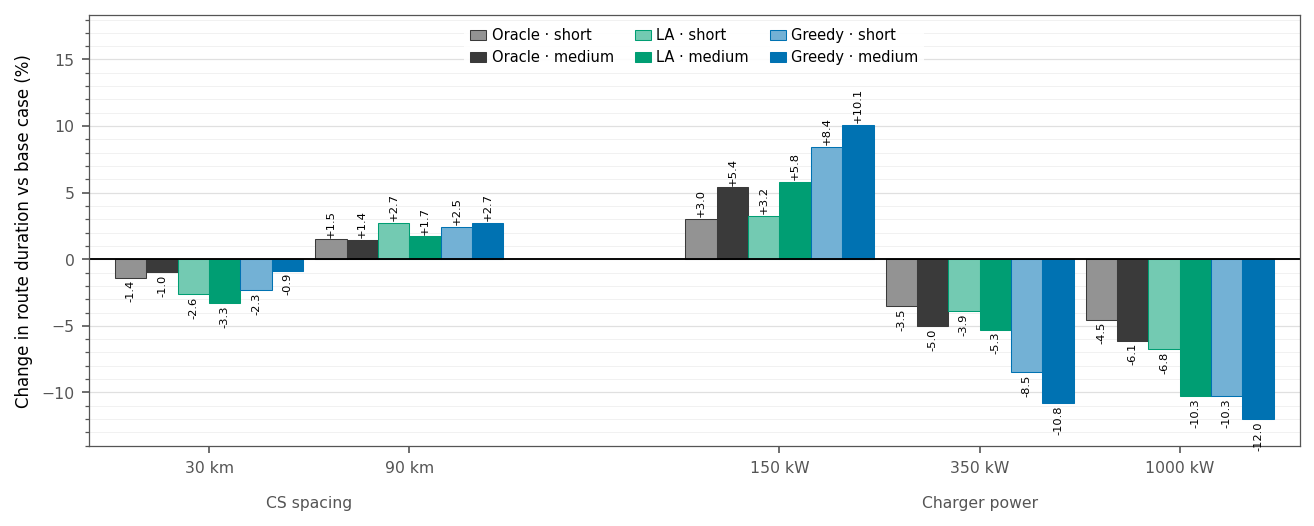
\includegraphics[width=0.8\linewidth]{figures/additional_sens_effects.png}
    \caption{One-at-a-time sensitivity of mean route duration to the charging
    infrastructure, relative to the base case, over the 160 paired instances of
    Section~\ref{sec:additional-protocol}.}
    \label{fig:sens}
\end{figure}

Charger power dominates charger density by roughly a factor of four over the
policy-relevant range.  Halving the AFIR spacing from 60 to 30\,km buys only
1.2\% of route duration at the hindsight optimum, while doubling it to 90\,km
costs 1.5\%: at the mandated spacing the corridor is already dense enough that
the binding constraint is how long a charging stop takes, not how far away the
next one is.  Upgrading the charger from the 200\,kW base to 350\,kW saves
4.2\%, and going all the way to a 1\,MW megawatt-charging system saves 5.3\%,
so a 350\,kW charger already captures four fifths of the benefit available at
five times the power.  Downgrading to 150\,kW costs 4.3\%.  The asymmetry is a
direct consequence of the concave charging curve: at low power the truck spends
its time in the slow final segment and adding power shortens exactly that
segment; once the fast segments are short relative to the mandatory rest
periods, extra power has nothing left to remove.  For a corridor already built
out to AFIR spacing, investment should therefore go into power per pool rather
than into more pools.

Two secondary observations are worth recording.  First, the effect is larger on
the medium routes than on the short ones on every power level ($-4.80$ vs.\
$-3.55$ at 350\,kW, $-6.02$ vs.\ $-4.53$ at 1\,MW), because a longer route
accumulates more charging events over which the saving compounds, whereas the
spacing effect is essentially route-length independent ($+1.46$ vs.\ $+1.55$ at
90\,km).  Second, Greedy over-reacts to the power axis by about a factor of two
relative to the oracle ($-9.61$ vs.\ $-4.17$ at 350\,kW).  This is a property
of the policy, not of the problem: Greedy charges to full whenever it stops, so
it sits on the slow tail of the charging curve far more often than an optimal
plan does, and it therefore benefits disproportionately from a faster charger.
An operator running without planning tools would over-estimate the value of a
charger upgrade by roughly a factor of two.


% ── DRAFT MARKER ────────────────────────────────────────────────────────────
% \PH{...} marks a number the sweep has not produced yet.  Delete this
% \providecommand once the last placeholder is gone.
\providecommand{\PH}[1]{\textbf{[#1]}}

\subsubsection{Look-ahead sensitivity}
\label{sec:la-config}

The LA policy has exactly two free parameters: the length $L$ of the rolling
look-ahead window and the number $|\Xi|$ of travel-time scenarios drawn at each
decision stop.  The base case of Section~\ref{sec:basecase} fixes them at
$L = 24$\,h and $|\Xi| = 25$.  Both are cost drivers, and they drive cost
differently: the per-decision workload grows roughly linearly in $|\Xi|$, since
the scenarios are evaluated independently, and faster than linearly in $L$,
since a longer window admits more stops and therefore more binaries into the
sub-problem.  Because LA re-solves at every stop, that cost is paid online, in
the cab, against the clock of a truck waiting to leave.  The configuration is
therefore a deployment decision rather than a tuning detail, and the question
this section answers is where the next second of on-board compute should go.

\paragraph{Protocol.}
This sweep departs from the protocol of
Section~\ref{sec:additional-protocol} in three ways, each forced by the
question.  First, it spans all three route classes, long ones included: the
whole point is how a truncated look-ahead behaves as the route outgrows it, so
excluding the case where truncation bites hardest would answer nothing.
Second, it fixes the customer count at medium and keeps only the \emph{none}
and \emph{tight} window classes, the two extremes of temporal coupling.  Third,
neither parameter changes the instance, so the runs are made on the base
instance files rather than on materialized copies; they consequently share the
existing hindsight-optimal cache, and every comparison is exactly paired on
geometry, customer draw \emph{and} travel-time realization.  With seeds
1--10 this gives $3 \times 2 \times 10 = 60$ instances per configuration.

Four configurations are taken one at a time off the base cell: $L \in
\{12, 48\}$\,h at $|\Xi| = 25$, and $|\Xi| \in \{10, 50\}$ at $L = 24$\,h.
Together with the base cell itself, which is the existing unlabelled LA runs on
these very instances, that is five cells and 300 runs.

\paragraph{Why these horizons.}
The horizon values are not a smooth grid, because the axis is not expected to
produce a smooth response.  Under the hours-of-service rules of
Section~\ref{sec:model}, a driver's day is bounded by a 13\,h spread that must
close with an 11\,h daily rest, so 24\,h is exactly one duty cycle.  A horizon
of 12\,h therefore ends before the current duty does and can never see the rest
that terminates it; 24\,h sees one complete cycle; 48\,h sees two.  If placing
a rest well requires seeing the end of the duty it closes, the response along
this axis is a threshold at the cycle length rather than a trend, and the
ladder is built to bracket that threshold from both sides.

Two structural remarks frame what follows.  The effective look-ahead is
$\min(L, \text{remaining route})$, so the axis saturates as soon as the horizon
covers the tail of the route.  Under the base configuration the median realized
duration is about 30\,h on the short routes, 58\,h on the medium ones and
109\,h on the long ones, so a 48\,h window already spans an entire short route
but never more than half a long one.  Route class is thus not a robustness
check here but the axis along which any horizon effect must appear, and its
absence on short routes would be a confirmation rather than a null result.  The
window class plays the analogous role for the scenario count: hours-of-service
coupling is deterministic given the realized travel times, whereas a time
window is a constraint on an uncertain arrival, so if scenarios buy anything
they should buy it under tight windows first.

\paragraph{Measures.}
Table~\ref{tab:la-config} reports each cell twice, and the two numbers answer
different questions.  The gap to the hindsight optimum is a \emph{level}: it
places a configuration against the best achievable schedule, but it inherits
the oracle's own residual optimality gap, which on long routes is structural
rather than incidental, so levels are comparable across configurations at a
fixed route class and should not be read across route classes.  The paired
$\Delta$ is the \emph{effect}: the median per-instance change in realized route
duration against the base cell.  Since both runs of a pair are policies on the
same instance and the same realization, the oracle cancels out of the
difference entirely, and this is the number the sweep is really about.  Cost is
reported as the median per-stop decision time rather than as wall clock, since
wall clock is only comparable across cells launched at the same concurrency and
would otherwise measure contention rather than compute.

One feature of the base cell is worth recording before the sweep, because it
conditions everything after it: tightening the windows roughly doubles the gap
to the hindsight optimum at every route class, while leaving the per-stop
decision time essentially unchanged.  The window constraint is where the online
policy loses most of its ground, and it costs LA nothing extra to solve.

% The generated file carries its own table environment, caption and label.
\begin{table}[htbp]\centering
\caption{Look-ahead configuration sensitivity.  Gap is the median gap to the hindsight optimum; $\Delta$ is the median paired change in route duration with respect to the base cell ($|\Xi| = 25$, $L = 24$\,h), positive meaning slower; $t_{\text{dec}}$ is the median per-stop decision time.  Cells shown as ``--'' have no runs yet.}
\label{tab:la-config}
\begin{tabular}{rrlrrrrrrrrr}
\toprule
\multicolumn{3}{c}{\textbf{Configuration}} & \multicolumn{3}{c}{\textbf{Short route}} & \multicolumn{3}{c}{\textbf{Medium route}} & \multicolumn{3}{c}{\textbf{Long route}} \\
\cmidrule(lr){1-3}\cmidrule(lr){4-6}\cmidrule(lr){7-9}\cmidrule(lr){10-12}
$|\Xi|$ & $L$ (h) & Windows & Gap (\%) & $\Delta$ (\%) & $t_{\text{dec}}$ (s) & Gap (\%) & $\Delta$ (\%) & $t_{\text{dec}}$ (s) & Gap (\%) & $\Delta$ (\%) & $t_{\text{dec}}$ (s) \\
\midrule
25 & 24 & None\rlap{\,\tiny base} & 2.0 & -- & 42 & 2.2 & -- & 78 & 2.4 & -- & 91 \\
25 & 24 & Tight\rlap{\,\tiny base} & 2.8 & -- & 51 & 3.6 & -- & 103 & 3.3 & -- & 100 \\
25 & 12 & None & 5.5 & +3.5 & 9 & 6.8 & +4.0 & 10 & 5.7 & +2.9 & 10 \\
25 & 12 & Tight & 9.7 & +5.1 & 10 & 9.6 & +3.3 & 11 & 7.7 & +2.9 & 11 \\
25 & 48 & None & 4.4 & +2.2 & 13 & 4.4 & +2.0 & 30 & 4.3 & +1.8 & 44 \\
25 & 48 & Tight & 8.2 & +3.0 & 15 & 8.5 & +2.5 & 34 & 5.3 & +2.0 & 50 \\
10 & 24 & None & 4.2 & +2.1 & 6 & 4.3 & +2.1 & 8 & 3.8 & +1.1 & 9 \\
10 & 24 & Tight & 7.7 & +2.8 & 6 & 6.1 & +2.0 & 8 & 5.0 & +1.2 & 9 \\
50 & 24 & None & 4.7 & +2.4 & 27 & 4.7 & +2.2 & 37 & 4.4 & +1.6 & 41 \\
50 & 24 & Tight & 8.0 & +3.0 & 29 & 7.3 & +2.8 & 40 & 5.2 & +1.6 & 43 \\
\bottomrule
\end{tabular}
\end{table}


\begin{figure}[htbp]
    \centering
    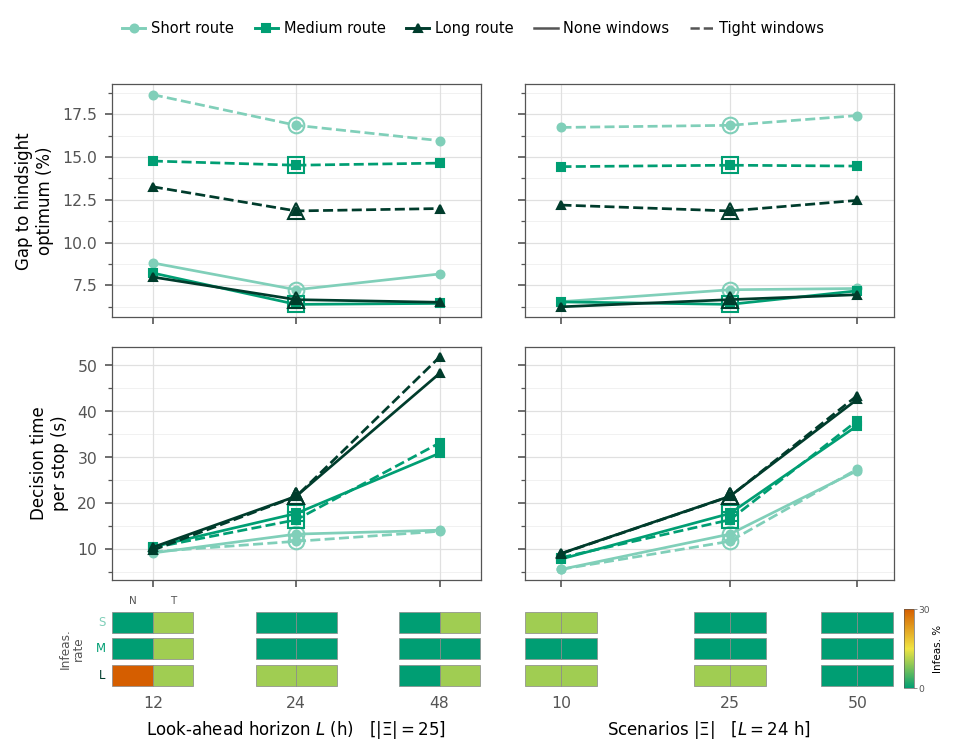
\includegraphics[width=\linewidth]{figures/additional_la_config.png}
    \caption{Look-ahead configuration sweep, one axis per column: horizon at
    the base scenario count (left) and scenario count at the base horizon
    (right).  Top row, distance to the hindsight optimum; bottom row, median
    per-stop decision time on a logarithmic scale.  Circled markers are the
    base cell, which lies on both ladders.  The dotted verticals mark the
    13\,h regular spread and the 24\,h duty cycle.}
    \label{fig:la-config}
\end{figure}

\begin{figure}[htbp]
    \centering
    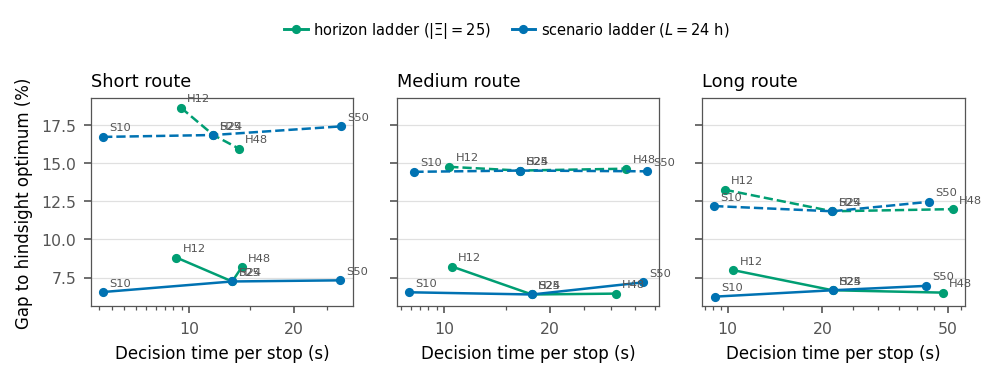
\includegraphics[width=\linewidth]{figures/additional_la_frontier.png}
    \caption{The same five cells plotted as cost against quality, one panel per
    route class.  The two ladders leave the base cell in different directions,
    and the steeper path identifies where an additional second of per-decision
    compute is better spent.}
    \label{fig:la-frontier}
\end{figure}

\paragraph{Results.}
\PH{The horizon axis.}  Shortening the window from 24\,h to 12\,h costs
\PH{$\Delta$ at each route class} and lengthening it to 48\,h changes the
realized duration by \PH{$\Delta$}, at \PH{factor} the decision time.
\PH{Whether the 12\,h penalty grows with route length, as the truncation
argument predicts, and whether 48\,h is flat against 24\,h.}

\PH{The scenario axis.}  Moving from 25 scenarios to 10 changes the realized
duration by \PH{$\Delta$} and to 50 by \PH{$\Delta$}, against a decision-time
ratio of \PH{factor} across that range.  \PH{Whether the effect is
concentrated under tight windows, as the coupling argument predicts.}

\PH{The trade-off.}  Read together (Figure~\ref{fig:la-frontier}),
\PH{which of the two ladders is steeper per second of decision time, and the
resulting recommendation for an on-board configuration}.

% ── INTERPRETATION, to be resolved against the numbers ──────────────────────
% Three readings are consistent with the design; the numbers decide between
% them.  Whichever holds, the paragraphs above should be rewritten as a claim,
% not as a hedge.
%
% (a) THRESHOLD.  L=12 is materially worse, L=48 indistinguishable from L=24,
%     and the L=12 penalty grows short -> medium -> long.  Claim: the horizon
%     must close one duty cycle and nothing beyond it is useful.  Decide on:
%     Delta(L=12) monotone in route class, and |Delta(L=48)| below the
%     seed-to-seed spread.
%
% (b) SATURATION ONLY.  L=12 costs little even on long routes.  Claim: the
%     rolling re-solve recovers what the shorter window gives up, and the
%     horizon can be halved for free -- a stronger deployment result than (a),
%     and it should be stated as such rather than buried.
%
% (c) SCENARIOS BUY CONSISTENCY, NOT LEVEL.  |Xi|=10 matches |Xi|=25 in the
%     median but has a heavier right tail.  Decide on the DISPERSION of the
%     paired deltas, not their median -- the current table reports medians
%     only, so if the medians coincide, add an IQR column and a box plot of
%     the paired deltas before concluding that scenarios do not matter.
%
% Also check before writing: n_infeasible per cell (a configuration that is
% faster because it strands the truck is not faster), and n_paired, which
% drops whenever either run of a pair is infeasible.
% ───────────────────────────────────────────────────────────────────────────


\subsubsection{Comparison with diesel trucks}
\label{sec:diesel}

To separate the cost of \emph{electrification} from the cost of
\emph{scheduling}, every instance of the subset in
Section~\ref{sec:additional-protocol} is re-solved as a diesel vehicle.  Diesel
mode removes the energy dimension entirely, that is per-leg consumption, the
battery and the charging curve, while keeping the node set, the customer windows
and the full Hours-of-Service machinery intact.  Former charging stations remain
as break-eligible waypoints, so the diesel problem is a genuine relaxation of
the electric one on the same corridor and the same travel-time realization, and
the two are solved by the same oracle and the same greedy policy.  The long
routes are included here on the Greedy comparison only.  Both oracles stall
there on the \emph{dual} bound, the electric one to 9.3\% and the diesel one
to 7.7\% within a two-hour budget, and the stall is driven by the rest-packing
structure rather than by the energy dimension, which is why removing the
battery does not relieve it.  A ratio of two loosely certified incumbents
compounds rather than cancels the two errors, so no hindsight optimum is
reported for that class; Greedy carries no optimality gap and is unaffected.

Of the station overheads, only the charger-specific ones are removed: the
queue, and the repositioning move off the charging bay before a break.  The
access manoeuvre is \emph{not}, because it is not charger-specific --- a diesel
driver taking a mandatory break also has to leave the motorway, park and
re-enter, and pays the same $M^{\text{stop}}$ for doing so.  Charging it to
only one of the two vehicles would credit the diesel with taking every one of
its breaks at no access cost, which overstates the electrification penalty by
roughly two percentage points and, as the decomposition below shows, misassigns
the single largest non-charging term.  All 160 instance pairs completed in both
worlds, and every oracle solve closed to within 0.5\%.

Refuelling is credited post hoc rather than modelled.  Unlike charging it has
no binding location choice, any truck stop serving, and on these corridors it
happens at most once: route lengths are 824--1219\,km (short) and
1541--2536\,km (medium) against a usable tank range of 1636--3240\,km across
the specifications in Table~\ref{tab:diesel-refuel}, so no fuel stop is
required on the short routes under any specification and at most one on the
medium routes.  We therefore credit the diesel with no fuel stop on the short
routes and one on the medium ones, at 19~minutes for access manoeuvre, queue
and pumping.  This is an assumption, not a derivation: the medium-route count
follows from the two smaller-tank specifications but not from the largest, and
crediting the stop lengthens the diesel makespan and so \emph{shrinks} the
reported penalty, by 0.67 percentage points.  Table~\ref{tab:diesel-refuel}
reports the zero-stop figures alongside, as the conservative bound.

\begin{table}[htbp]
\centering
\caption{Electric versus diesel route duration on identical instances and
realizations.  ``Coupling'' is the share of charging time credited inside a
mandatory break, $\sum_i g_i / \sum_i \tau^c_i$, at the hindsight optimum.
``EV cert.'' is the worst remaining MIP gap on the electric oracle: where it
exceeds the solver tolerance the electric schedule is an incumbent rather than
a proven optimum, so the penalty is an upper bound on the true optimal one.
$n = 80$ instances per route class.}
\label{tab:diesel}
\begin{tabular}{lrrrrrr}
\toprule
\textbf{Route} & \textbf{Diesel (h)} & \textbf{EV (h)} & \textbf{Charging (h)}
 & \textbf{Oracle (\%)} & \textbf{Greedy (\%)} & \textbf{Coupling (\%)} \\
\midrule
Short  & 26.6 & 28.7 & 2.69 & $+8.0$ & $+20.0$ & 76 \\
Medium & 53.2 & 58.2 & 6.80 & $+9.4$ & $+23.0$ & 70 \\
Long   & --   & --   & --   & --     & $+21.0$ & -- \\
\bottomrule
\end{tabular}
\end{table}

\begin{figure}[htbp]
    \centering
    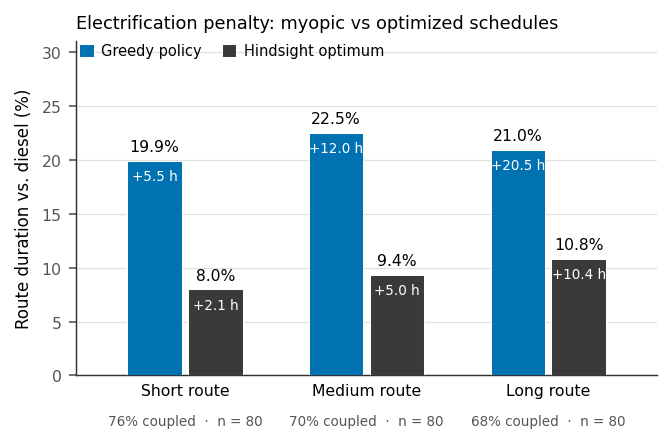
\includegraphics[width=0.75\linewidth]{figures/additional_diesel_gap.png}
    \caption{Electrification penalty in route duration, per route class: the
    penalty realized by the greedy policy against the one realized by the
    hindsight optimum.  The annotation below each group gives the mean coupling
    share $\sum_i g_i/\sum_i \tau^c_i$ and the number of instances.}
    \label{fig:diesel}
\end{figure}

Electrification carries a real and irreducible makespan penalty on these
corridors: $+8.0\%$ on the short routes and $+9.4\%$ on the medium ones at the
hindsight optimum, positive on every one of the 160 instances (range $+2.2$ to
$+25.3\%$).  Break/charge coupling is effective in the sense the model
predicts, since 70--76\% of charging time is credited inside a mandatory break,
but it is far from cancelling the cost of charging.  Decomposing the penalty
shows why.  Both schedules are broken into
the terms of their own departure equations and differenced; driving is identical
within each pair, so the modelled rows below close the gap exactly, and the
diesel's fuel stop is then credited against that subtotal:

\begin{center}
\begin{tabular}{lrr}
\toprule
 & \textbf{Short (h)} & \textbf{Medium (h)} \\
\midrule
Total charging time                   & $+2.69$ & $+6.80$ \\
Charging-station queueing             & $+0.33$ & $+0.78$ \\
Stop manoeuvring, net of diesel       & $+0.37$ & $+0.63$ \\
Repositioning off the charging bay    & $+0.01$ & $+0.06$ \\
Break time no longer taken separately & $-1.25$ & $-3.19$ \\
Rest time                             & $-0.06$ & $+0.20$ \\
\midrule
Modelled subtotal                     & $+2.09$ & $+5.28$ \\
Diesel refuelling (post hoc)          & $-0.00$ & $-0.32$ \\
\midrule
\textbf{Net penalty vs.\ diesel}      & $\mathbf{+2.09}$ & $\mathbf{+4.97}$ \\
\bottomrule
\end{tabular}
\end{center}

The coupling credit, that is the break time the driver no longer has to take
separately, is 1.25\,h and 3.19\,h, but it is bounded above by the break
duration that the regulation requires in the first place: charging for longer
than 45~minutes at a stop earns no further credit.  Against it the electric
truck pays 0.71\,h and 1.47\,h of station access that the diesel does not: the
queue, the bay repositioning, and the residual manoeuvring of the stops it makes
\emph{only} to charge.  Note how small that last term is once the diesel is
charged for its own break access --- the manoeuvring row falls from 0.55\,h and
1.38\,h in absolute terms to 0.37\,h and 0.63\,h net, so roughly half of what
looks like an electric access penalty is simply the cost of stopping, which any
vehicle subject to the same break regime pays.  The genuinely electric access
overhead nonetheless consumes about half the coupling credit, so barely half of
the credit survives to offset the charging time itself.  This qualifies, rather
than contradicts, the finding of
\citet{brockmann_break-and-charge_2025} that mandatory breaks create natural
charging windows: the windows exist and the model exploits them, but the access
overheads of a fast-charging stop, which that work does not price, absorb a
substantial part of the gain.

The greedy comparison isolates the remaining half of the story, and it is the
only one available on the long routes.  Greedy's electric schedule is 20.0\%
longer than its own diesel schedule on the short routes, 23.0\% longer on the
medium ones and 21.0\% longer on the long ones ($n = 67$; the remainder are
instances where the myopic rule violates Hours-of-Service in one world or the
other and is recorded as infeasible).  The penalty is thus flat in route
length once the corridor is long enough to be rest-dominated.  On the two
classes where the optimum is certified this is about two and a half times the
optimal penalty.  The excess is not electrification but planning quality:
measured against its own hindsight optimum, Greedy loses 13.2\% (short) and
14.4\% (medium) on the electric problem, but only 2.1\% and 1.6\% on the diesel
problem, where the myopic rule is nearly optimal because the sole remaining
decision is when to rest.  Electrification is thus what turns a scheduling
problem that a rule of thumb solves almost optimally into one where a rule of
thumb costs a further 11--13 percentage points of makespan.  Of the roughly
20--23\% that an operator would observe when switching a myopically-scheduled
corridor from diesel to battery-electric, about half is the physical cost of
charging and about half would be recovered by adopting a planner such as the
ones compared in Section~\ref{sec:basecase}.

\begin{figure}[htbp]
    \centering
    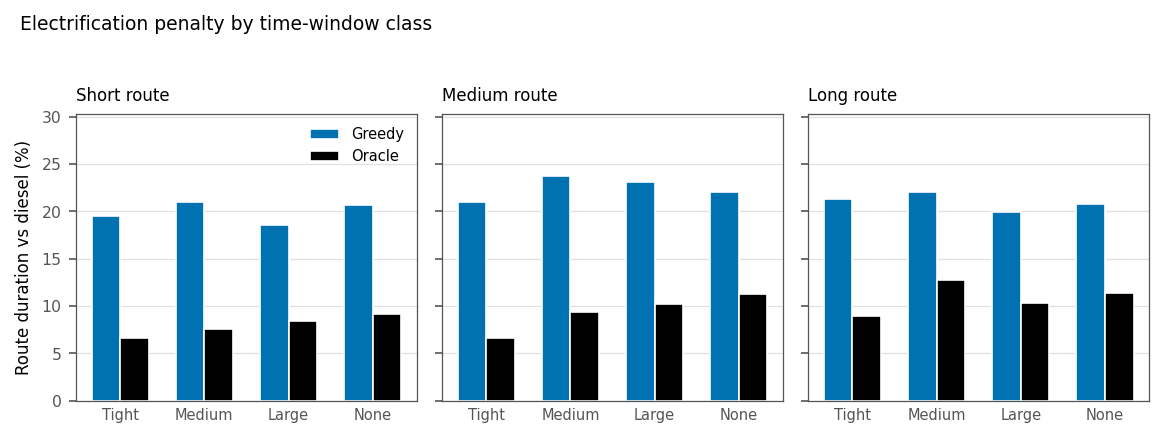
\includegraphics[width=\linewidth]{figures/additional_diesel_tw.png}
    \caption{Electrification penalty by time-window class.  The optimized
    penalty rises monotonically as windows loosen; the myopic one does not
    respond to windows at all.  Long routes carry no certified oracle
    (Section~\ref{sec:diesel}), so only Greedy is shown there.}
    \label{fig:diesel-tw}
\end{figure}

The penalty is not uniform across window classes, and the variation identifies
its mechanism.  At the hindsight optimum it rises monotonically as windows
loosen, from $+6.7\%$ to $+9.2\%$ on the short routes and from $+6.6\%$ to
$+11.3\%$ on the medium ones (Figure~\ref{fig:diesel-tw},
Table~\ref{tab:diesel-tw}), while the Greedy penalty is flat in the window
class on all three route classes.  What changes is not the electric truck.  It
takes \emph{zero} standalone break time in every single cell, charging through
every break the regulation requires, and its coupling share stays between 68
and 80\% throughout.  What changes is the diesel.  Idle waiting is disabled, so
a vehicle arriving before a window opens must either stretch a break or accept
the out-of-window penalty, and the diesel, being the faster of the two, is the
one that arrives early: 30 of its 35 out-of-window service starts are early
arrivals, against none of the electric truck's seven, which are all late.  Its
standalone break time accordingly rises from 2.74\,h under no windows to
3.90\,h under tight ones on the medium routes, while the electric truck, parked
at a charger for that break in either case, absorbs the same delay for free.
Tight windows do not make electrification cheaper; they make the diesel's speed
advantage unusable.

This is a makespan comparison throughout, and the window penalty does not drive
it.  Charging each vehicle $\beta_{TW}$ per missed window changes the ordering
nowhere and the magnitude by at most 1.9 percentage points --- on the medium
routes under medium windows, where the diesel misses 0.95 windows per instance
on average against the electric truck's zero --- and the monotone trend
survives unchanged.


\subsubsection{Effect of uncertainty}
\label{sec:uncertainty}

The final block isolates what uncertainty itself costs, along three lines: what
it does to window compliance, how much of the loss can be recovered by adapting
en route, and how much would remain even with perfect information.

First, uncertainty is paid in windows, not in driving time.  This is already
visible in the base case, without any additional run.  The two gap definitions
reported in Table~\ref{tab:gap} differ only by the
$\beta\sum_i\delta_i$ term, and their difference is concentrated exactly where
uncertainty has the most to disrupt: on the window-free classes the two coincide
to the last digit, whereas on the tight-window classes the penalty term accounts
for 25\% of RO's gap, 38\% of SP's, 38\% of Greedy's, 38\% of LA's and 43\% of
ROBU's, rising to two thirds for Greedy on
\emph{Short}/\emph{Many}/\emph{Tight}.  Window compliance is also the axis on
which the methods separate most: 41.2\% (RO), 55.1\% (Greedy), 67.0\% (LA),
67.3\% (ROBU), 84.8\% (SP) in Table~\ref{tab:feasibility}, against a spread of
under two percentage points in HoS violations.  A schedule committed before
departure survives the travel-time noise in its rest structure and fails in its
appointments.

Second, adapting en route recovers most of that loss, and the price of the
adaptation differs sharply between the two adaptive architectures.  SP reaches
its 84.8\% window hit rate by repairing its committed structure on 99.0\% of
executions and pays for it with a 12.0\% stranding rate; LA reaches 67.0\% with
no recourse machinery at all, at 14--22\,s of re-optimisation per stop and a
1.4\% stranding rate.  The comparison across route classes in
Table~\ref{tab:gap} sharpens this: full re-optimisation at every stop degrades
gracefully with route length (11.7\%, 12.9\%, 10.9\% mean gap on short, medium
and long), whereas a scenario set fixed at departure is excellent on the short
routes (4.9\%), no better than LA on the medium ones (12.9\%), and unusable on
the long ones.  The value of re-planning is therefore not uniform: it grows with
the horizon over which the initial scenario set becomes stale.

Finally we decompose the total cost of uncertainty on a common set of scenarios,
drawn once per instance with common random numbers so that all three legs see
identical realizations.  Let WS be the mean perfect-hindsight optimum over the
scenario set (wait-and-see); RP the mean realized objective of the two-stage
plan executed with online duration recourse; and EEV the mean realized objective
of the plan obtained from the expected-value problem, that is the deterministic
model solved at nominal travel times, executed under the same recourse
semantics.  Then
\begin{equation}
\mathrm{VSS} = \mathrm{EEV} - \mathrm{RP}, \qquad
\mathrm{EVPI} = \mathrm{RP} - \mathrm{WS},
\end{equation}
where VSS measures what modelling the travel-time distribution at plan time is
worth relative to planning on the mean, and EVPI the irreducible loss that no
amount of distributional modelling can recover.  Because the two-stage plan is
taken from the base-case SP runs, its scenarios are not the common-random ones
and the RP leg is consequently a slight over-estimate; this is flagged in the
table note.

\begin{table}[htbp]
\centering
\caption{Value of the stochastic solution (VSS) and expected value of perfect
information (EVPI), over common-random scenarios, by instance class.
$\mathrm{VSS} = \mathrm{EEV} - \mathrm{RP}$ and
$\mathrm{EVPI} = \mathrm{RP} - \mathrm{WS}$, in hours of route duration.}
\label{tab:vss}
\begin{tabular}{lrrrrrr}
\toprule
\textbf{Class} & \textbf{WS (h)} & \textbf{RP (h)} & \textbf{EEV (h)} & \textbf{VSS (h)} & \textbf{EVPI (h)} & \textbf{n} \\
\midrule
RshortCfew   & \red{--} & \red{--} & \red{--} & \red{--} & \red{--} & \red{--} \\
RshortCmany  & \red{--} & \red{--} & \red{--} & \red{--} & \red{--} & \red{--} \\
RmediumCfew  & \red{--} & \red{--} & \red{--} & \red{--} & \red{--} & \red{--} \\
RmediumCmany & \red{--} & \red{--} & \red{--} & \red{--} & \red{--} & \red{--} \\
\bottomrule
\end{tabular}
\end{table}

\red{Table~\ref{tab:vss} is still a skeleton: the harness
(\texttt{experiments/vss\_evpi.py}) is implemented and wired into
\texttt{additional\_analysis.py vss}, but no instance has been run.  Each
instance costs $1 + n_{\mathrm{scen}}$ oracle solves (one expected-value solve
plus one wait-and-see solve per scenario), so at 20 scenarios the four classes
above are the practical limit.  Run with
\texttt{python additional\_analysis.py vss -{}-n-scenarios 20}, then
\texttt{python additional\_figures.py -{}-section vss}.}
